\documentclass[12pt]{article}
\usepackage[margin=2cm]{geometry}
\usepackage{amsmath}
\usepackage{slashed}
\usepackage{tikz}

\begin{document}

\noindent
Compton scattering occurs when a high energy photon such as a gamma ray interacts with an electron.
In typical Compton scattering experiments the incident electron is at rest with zero velocity.
However, it is easier to develop a theory using the center of mass frame in which
the photon and the electron have equal and opposite momentum.
The following diagram shows the photon and electron scattering through angle $\theta$
in the center of mass frame.
\begin{center}
\begin{tikzpicture}
\draw[dashed] (0,0) circle (0.5cm);
\draw[thick,->] (2,0) node[anchor=west] {$e^-$} -- (0.6,0);
\draw[thick,->] (-2,0) node[anchor=east] {$\gamma$} -- (-0.6,0);
\draw[thick,->] (0.40,0.40) -- (1.3,1.3) node[anchor=south west] {$\gamma$};
\draw[thick,->] (-0.4,-0.4) -- (-1.3,-1.3) node[anchor=north east] {$e^-$};
\draw (1,0.5) node {$\theta$};
\end{tikzpicture}
\end{center}

\noindent
Here is the same diagram with momentum and spinor labels.
\begin{center}
\begin{tikzpicture}
\draw[dashed] (0,0) circle (0.5cm);
\draw[thick,->] (2,0) node[anchor=west] {$p_2, u_2$} -- (0.6,0);
\draw[thick,->] (-2,0) node[anchor=east] {$p_1$} -- (-0.6,0);
\draw[thick,->] (0.40,0.40) -- (1.3,1.3) node[anchor=south west] {$p_3$};
\draw[thick,->] (-0.4,-0.4) -- (-1.3,-1.3) node[anchor=north east] {$p_4, u_4$};
\draw (1,0.5) node {$\theta$};
\end{tikzpicture}
\end{center}

\noindent
In center of mass coordinates the momentum vectors are
\begin{equation*}
\underset{\text{inbound photon}}
{
p_1=\begin{pmatrix}\omega\\0\\0\\ \omega\end{pmatrix}
}
\qquad
\underset{\text{inbound electron}}
{
p_2=\begin{pmatrix}E\\0\\0\\-\omega\end{pmatrix}
}
\qquad
\underset{\text{outbound photon}}
{
p_3=\begin{pmatrix}
\omega\\
\omega\sin\theta\cos\phi\\
\omega\sin\theta\sin\phi\\
\omega\cos\theta
\end{pmatrix}
}
\qquad
\underset{\text{outbound electron}}
{
p_4=\begin{pmatrix}
E\\
-\omega\sin\theta\cos\phi\\
-\omega\sin\theta\sin\phi\\
-\omega\cos\theta
\end{pmatrix}
}
\end{equation*}

\noindent
Symbol $\omega$ is incident momentum,
$E$ is total energy $E=\sqrt{\omega^2+m^2}$,
and $m$ is electron mass.
Polar angle $\theta$ is the observed scattering angle.
Azimuth angle $\phi$ cancels out in scattering calculations.

\bigskip
\noindent
The spinors are
\begin{equation*}
\underset{\text{inbound electron, spin up}}
{
u_{21}=\begin{pmatrix}
E+m\\
0\\
-\omega\\
0
\end{pmatrix}
}
\qquad
\underset{\text{inbound electron, spin down}}
{
u_{22}=\begin{pmatrix}
0\\
E+m\\
0\\
\omega
\end{pmatrix}
}
\qquad
\underset{\text{outbound electron, spin up}}
{
u_{41}=\begin{pmatrix}
E+m\\
0\\
p_{4z}\\
p_{4x}+ip_{4y}
\end{pmatrix}
}
\qquad
\underset{\text{outbound electron, spin down}}
{
u_{42}=\begin{pmatrix}
0\\
E+m\\
p_{4x}-ip_{4y}\\
-p_{4z}
\end{pmatrix}
}
\end{equation*}

\noindent
The spinors shown above are not individually normalized.
Instead, a combined spinor normalization constant $N=(E+m)^2$ will be used.

\bigskip
\noindent
The following formula computes a probability density $|\mathcal{M}_{ab}|^2$
for Compton scattering where $a$ is the spin state of the inbound electron
and $b$ is the spin state of the outbound electron.
\begin{equation*}
|\mathcal{M}_{ab}|^2
=
\frac{e^4}{N}
\left|
-\frac{\bar{u}_{4b}\gamma^\mu(\slashed{q}_1+m)\gamma^\nu u_{2a}}{s-m^2}
-\frac{\bar{u}_{4b}\gamma^\nu(\slashed{q}_2+m)\gamma^\mu u_{2a}}{u-m^2}
\right|^2
\end{equation*}
Symbol $e$ is electron charge.
Symbols $s$ and $u$ are Mandelstam variables $s=(p_1+p_2)^2$ and $u=(p_1-p_4)^2$.
Symbol $q_1=p_1+p_2$ and $q_2=p_2-p_3$.

\bigskip
\noindent
Let
\begin{equation*}
a_1=\bar{u}_{4b}\gamma^\mu(\slashed{q}_1+m)\gamma^\nu u_{2a}
\qquad
a_2=\bar{u}_{4b}\gamma^\nu(\slashed{q}_2+m)\gamma^\mu u_{2a}
\end{equation*}

\noindent
Then
\begin{align*}
|\mathcal{M}_{ab}|^2&=\frac{e^4}{N}\left|-\frac{a_1}{s-m^2}-\frac{a_2}{u-m^2}\right|^2\\
&=
\frac{e^4}{N}
\left(-\frac{a_1}{s-m^2}-\frac{a_2}{u-m^2}\right)
\left(-\frac{a_1}{s-m^2}-\frac{a_2}{u-m^2}\right)^*\\
&=
\frac{e^4}{N}\left(
\frac{a_1a_1^*}{(s-m^2)^2}
+\frac{a_1a_2^*}{(s-m^2)(u-m^2)}
+\frac{a_1^*a_2}{(s-m^2)(u-m^2)}
+\frac{a_2a_2^*}{(u-m^2)^2}
\right)
\end{align*}

\noindent
The expected probability density $\langle|\mathcal{M}|^2\rangle$ is
computed by summing $|\mathcal{M}_{ab}|^2$ over all spin and polarization states
and then dividing by the number of inbound states.
There are four inbound states.
The sum over polarizations is already accomplished by contraction of $aa^*$ over $\mu$ and $\nu$.
\begin{align*}
\langle|\mathcal{M}|^2\rangle
&=\frac{1}{4}\sum_{a=1}^2\sum_{b=1}^2|\mathcal{M}_{ab}|^2\\
&=\frac{e^4}{4}\sum_{a=1}^2\sum_{b=1}^2
\frac{1}{N}\left(
\frac{a_1a_1^*}{(s-m^2)^2}
+\frac{a_1a_2^*}{(s-m^2)(u-m^2)}
+\frac{a_1^*a_2}{(s-m^2)(u-m^2)}
+\frac{a_2a_2^*}{(u-m^2)^2}
\right)
\end{align*}

\noindent
Use the Casimir trick to replace sums over spins with matrix products.
\begin{align*}
f_{11}&=\frac{1}{N} \sum_{a=1}^2\sum_{b=1}^2 a_1a_1^*=\mathop{\rm Tr}
\left(
(\slashed{p}_2+m)\gamma^\mu(\slashed{q}_1+m)\gamma^\nu(\slashed{p}_4+m)\gamma_\nu(\slashed{q}_1+m)\gamma_\mu
\right)
\\
f_{12}&=\frac{1}{N} \sum_{a=1}^2\sum_{b=1}^2 a_1a_2^*=\mathop{\rm Tr}
\left(
(\slashed{p}_2+m)\gamma^\mu(\slashed{q}_2+m)\gamma^\nu(\slashed{p}_4+m)\gamma_\mu(\slashed{q}_1+m)\gamma_\nu
\right)
\\
f_{22}&=\frac{1}{N} \sum_{a=1}^2\sum_{b=1}^2 a_2a_2^*=\mathop{\rm Tr}
\left(
(\slashed{p}_2+m)\gamma^\mu(\slashed{q}_2+m)\gamma^\nu(\slashed{p}_4+m)\gamma_\nu(\slashed{q}_2+m)\gamma_\mu
\right)
\end{align*}

\noindent
Hence
\begin{equation}
\langle|\mathcal{M}|^2\rangle
=
\frac{e^4}{4}
\left(
\frac{f_{11}}{(s-m^2)^2}
+\frac{f_{12}}{(s-m^2)(u-m^2)}
+\frac{f_{12}^*}{(s-m^2)(u-m^2)}
+\frac{f_{22}}{(u-m^2)^2}
\right)
\end{equation}

\noindent
Run ``compton-scattering-1.txt'' to verify the Casimir trick for Compton scattering.

\bigskip
\noindent
The following momentum formulas are equivalent to the Casimir trick.
(Recall that $a\cdot b=a^\mu g_{\mu\nu}b^\nu$)
\begin{align*}
f_{11}&=
-16 (p_1 \cdot p_1) (p_2 \cdot p_4) +
 32 (p_1 \cdot p_2) (p_1 \cdot p_4) +
 32 (p_1 \cdot p_4) (p_2 \cdot p_2) +
 16 (p_2 \cdot p_2) (p_2 \cdot p_4) %+
\\ &\phantom{=}\qquad{}+
 64 m^2 (p_1 \cdot p_1) +
 64 m^2 (p_1 \cdot p_2) -
 64 m^2 (p_1 \cdot p_4) -
 48 m^2 (p_2 \cdot p_4) + 64 m^4
\\
f_{12}&=
-32 (p_1 \cdot p_2) (p_2 \cdot p_4) +
 32 (p_1 \cdot p_3) (p_2 \cdot p_4) -
 32 (p_2 \cdot p_2) (p_2 \cdot p_4) +
 32 (p_2 \cdot p_3) (p_2 \cdot p_4) %+
 \\ &\phantom{=}\qquad{}+
 32 m^2 (p_1 \cdot p_2) -
 16 m^2 (p_1 \cdot p_3) +
 16 m^2 (p_1 \cdot p_4) %+
 \\ &\phantom{=}\qquad{}+
 48 m^2 (p_2 \cdot p_2) -
 32 m^2 (p_2 \cdot p_3) +
 48 m^2 (p_2 \cdot p_4) -
 16 m^2 (p_3 \cdot p_4) - 32 m^4
\\
f_{22}&=
16 (p_2 \cdot p_2) (p_2 \cdot p_4) -
32 (p_2 \cdot p_2) (p_3 \cdot p_4) +
32 (p_2 \cdot p_3) (p_3 \cdot p_4) -
16 (p_2 \cdot p_4) (p_3 \cdot p_3) %-\\
\\ &\phantom{=}\qquad{}-
64 m^2 (p_2 \cdot p_3) -
48 m^2 (p_2 \cdot p_4) +
64 m^2 (p_3 \cdot p_3) +
64 m^2 (p_3 \cdot p_4) + 64 m^4
\end{align*}

\noindent
Using Mandelstam variables
\begin{align*}
s&=(p_1+p_2)^2
\\
t&=(p_1-p_3)^2
\\
u&=(p_1-p_4)^2
\end{align*}
the momentum formulas are
\begin{equation}
\begin{aligned}
f_{11}&=-8 s u + 24 s m^2 + 8 u m^2 + 8 m^4
\\
f_{12}&=8 s m^2 + 8 u m^2 + 16 m^4
\\
f_{22}&=-8 s u + 8 s m^2 + 24 u m^2 + 8 m^4
\end{aligned}
\end{equation}

\noindent
Run ``compton-scattering-2.txt'' to verify momentum formulas for Compton scattering.

\subsection*{High energy approximation}
For high energy experiments that have $\omega\gg m$ the approximation $m=0$ can be used
resulting in the following simplified probability density.
\begin{align*}
\langle|\mathcal{M}|^2\rangle
&=\frac{e^4}{4}
\left(\frac{-8su}{s^2}+\frac{-8su}{u^2}\right)
\\
&=2e^4
\left(-\frac{u}{s}-\frac{s}{u}\right)
\end{align*}

\noindent
Also for $m=0$ the Mandelstam variables $s$ and $u$ are
\begin{align*}
s&=4\omega^2
\\
u&=-2\omega^2(1+\cos\theta)
\end{align*}
Hence
\begin{equation}
\langle|\mathcal{M}|^2\rangle
=2e^4\left(
\frac{1+\cos\theta}{2}+\frac{2}{1+\cos\theta}
\right)
\end{equation}

\subsection*{Lab frame}
Compton scattering experiments are typically done in the ``lab'' frame where the electron is at rest.
The following Lorentz boost $\Lambda$ transforms momentum vectors from
the center of mass frame to the lab frame.
\begin{equation*}
\Lambda=
\begin{pmatrix}
E/m & 0 & 0 & \omega/m\\
0 & 1 & 0 & 0\\
0 & 0 & 1 & 0\\
\omega/m & 0 & 0 & E/m
\end{pmatrix},
\qquad
\Lambda p_2=\begin{pmatrix}m \\ 0 \\ 0 \\ 0\end{pmatrix}
\end{equation*}

\noindent
Mandelstam variables are invariant under a boost.
\begin{equation*}
\begin{aligned}
s&=(p_1+p_2)^2=(\Lambda p_1+\Lambda p_2)^2
\\
t&=(p_1-p_3)^2=(\Lambda p_1-\Lambda p_3)^2
\\
u&=(p_1-p_4)^2=(\Lambda p_1-\Lambda p_4)^2
\end{aligned}
\end{equation*}

\noindent
In the lab frame, let $\omega_L$ be the angular frequency of the incident photon
and let $\omega_L'$ be the angular frequency of the scattered photon.
\begin{equation*}
\begin{aligned}
\omega_L&=\Lambda p_1\cdot(1,0,0,0)=\frac{\omega^2}{m}+\frac{\omega E}{m}
\\
\omega_L'&=\Lambda p_3\cdot(1,0,0,0)=\frac{\omega^2\cos\theta}{m}+\frac{\omega E}{m}
\end{aligned}
\end{equation*}

\noindent
It follows that
\begin{equation*}
\begin{aligned}
s&=(p_1+p_2)^2=2m\omega_L+m^2
\\
t&=(p_1-p_3)^2=2m(\omega_L' - \omega_L)
\\
u&=(p_1-p_4)^2=-2 m \omega_L' + m^2
\end{aligned}
\end{equation*}

\noindent
Compute $\langle|\mathcal{M}|^2\rangle$ using equations (1) and (2)
and the above $s$, $t$, and $u$ that involve $\omega_L$ and $\omega_L'$.
\begin{equation*}
\langle|\mathcal{M}|^2\rangle=
2e^4\left(
\frac{\omega_L}{\omega_L'}+\frac{\omega_L'}{\omega_L}
+\left(\frac{m}{\omega_L}-\frac{m}{\omega_L'}+1\right)^2-1
\right)
\end{equation*}

\noindent
From the Compton formula
\begin{equation*}
\frac{1}{\omega_L'}-\frac{1}{\omega_L}=\frac{1-\cos\theta_L}{m}
\end{equation*}

\noindent
we have
\begin{equation*}
\cos\theta_L=\frac{m}{\omega_L}-\frac{m}{\omega_L'}+1
\end{equation*}

\noindent
Hence
\begin{equation*}
\langle|\mathcal{M}|^2\rangle=
2e^4\left(
\frac{\omega_L}{\omega_L'}+\frac{\omega_L'}{\omega_L}+\cos^2\theta_L-1
\right)
\end{equation*}

\noindent
Run ``compton-scattering-3.txt'' to verify lab frame formulas for Compton scattering.

\subsection*{Cross section}
Now that we have derived $\langle|\mathcal{M}|^2\rangle$
we can investigate the angular distribution of scattered photons.
For simplicity let us drop the $L$ subscript from lab variables.
From now on the symbols $\omega$, $\omega'$, and $\theta$ will be lab frame variables.

\bigskip
\noindent
The differential cross section for Compton scattering is
\begin{align*}
\frac{d\sigma}{d\Omega}&=\frac{\hbar^2}{64\pi^2m^2c^4}
\left(\frac{\omega'}{\omega}\right)^2\langle|\mathcal{M}|^2\rangle
\\
&=\frac{e^4\hbar^2}{32\pi^2m^2c^4}
\left(\frac{\omega'}{\omega}\right)^2
\left(
\frac{\omega}{\omega'}+\frac{\omega'}{\omega}+\cos^2\theta-1
\right)
\end{align*}

\noindent
From $e^4=16\pi^2\alpha^2$ we have
\begin{equation*}
\frac{d\sigma}{d\Omega}
=\frac{\alpha^2\hbar^2}{2m^2c^4}
\left(\frac{\omega'}{\omega}\right)^2
\left(
\frac{\omega}{\omega'}+\frac{\omega'}{\omega}+\cos^2\theta-1
\right)
\end{equation*}

\noindent
The scattered photon frequency $\omega'$ is computed from the Compton equation.
\begin{equation*}
\omega'=\frac{m\omega}{m+\omega(1-\cos\theta)}
\end{equation*}

\noindent
We can integrate $d\sigma$ to obtain a cumulative distribution function.
Recall that
\begin{equation*}
d\Omega=\sin\theta\,d\theta\,d\phi
\end{equation*}
Hence
\begin{equation*}
d\sigma
=\frac{\alpha^2\hbar^2}{2m^2c^4}
\left(\frac{\omega'}{\omega}\right)^2
\left(\frac{\omega}{\omega'}+\frac{\omega'}{\omega}+\cos^2\theta-1\right)
\sin\theta\,d\theta\,d\phi
\end{equation*}

\bigskip
\noindent
Let $I(\theta)$ be the following integral of $d\sigma$.
\begin{align*}
I(\theta)
&=\left(\frac{2m^2c^4}{\alpha^2\hbar^2}\right)\frac{1}{2\pi}\int_0^{2\pi}\int d\sigma
\\
&=\int
\left(\frac{\omega'}{\omega}\right)^2
\left(\frac{\omega}{\omega'}+\frac{\omega'}{\omega}+\cos^2\theta-1\right)
\sin\theta\,d\theta,
\quad0\le\theta\le\pi
\end{align*}

\noindent
Assume that $I(\theta)-I(0)$ is computable given $\theta$ by either symbolic or numerical integration.

\bigskip
\noindent
Let $C$ be the normalization constant
\begin{equation*}
C=I(\pi)-I(0)
\end{equation*}

\noindent
Then the cumulative distribution function $F(\theta)$ is
\begin{equation*}
F(\theta)=\frac{I(\theta)-I(0)}{C},
\quad0\le\theta\le\pi
\end{equation*}

\noindent
The probability of observing scattering events in the interval
$\theta_1$ to $\theta_2$ can now be computed.
\begin{equation*}
P(\theta_1\le\theta\le\theta_2)=F(\theta_2)-F(\theta_1)
\end{equation*}

\noindent
The probability density function $f(\theta)$ is the derivative of $F(\theta)$.
\begin{equation*}
f(\theta)=\frac{dF(\theta)}{d\theta}
=\frac{1}{C}
\left(\frac{\omega'}{\omega}\right)^2
\left(\frac{\omega}{\omega'}+\frac{\omega'}{\omega}+\cos^2\theta-1\right)
\sin\theta
\end{equation*}

\noindent
Run ``compton-scattering-4.txt'' to draw a graph of $f(\theta)$ for
$\omega=500\,\text{keV}=1.2\times10^{20}\,\text{Hz}$.

\begin{center}
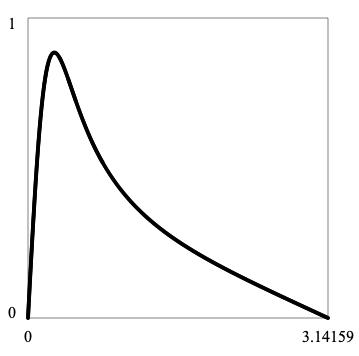
\includegraphics[scale=0.5]{compton-scattering.png}
\end{center}

\noindent
Probability distribution for $45^\circ$ bins
($\omega=500\,\text{keV}=1.2\times10^{20}\,\text{Hz}$).

\begin{center}
\begin{tabular}{|c|c|c|}
\hline
$\theta_1$ & $\theta_2$ & $P(\theta_1\le\theta\le\theta_2)$\\
\hline
$0^\circ$ & $45^\circ$ & 0.35 \\
$45^\circ$ & $90^\circ$ & 0.34 \\
$90^\circ$ & $135^\circ$ & 0.22 \\
$135^\circ$ & $180^\circ$ & 0.09 \\
\hline
\end{tabular}
\end{center}

\subsection*{Thomson scattering}
When $\omega$ is much smaller than the electron mass $m$ we have
\begin{equation*}
\frac{m}{m+\omega(1-\cos\theta)}\approx1
\end{equation*}

\noindent
Hence for $\omega\ll m$ the differential cross section is approximately
\begin{equation*}
\frac{d\sigma}{d\Omega}=\frac{\alpha^2}{2m^2}(1+\cos^2\theta)
\end{equation*}

\noindent
which is the formula for Thomson scattering.

\subsection*{Data from a CERN LEP experiment}
See ``Compton Scattering of Quasi-Real Virtual Photons at LEP,''
arxiv.org/abs/hep-ex/0504012.

\begin{center}
\begin{tabular}{|c|c|}
\hline
$x$ & $y$\\
\hline
$-0.74$ & $13380$\\
$-0.60$ & $\phantom{0}7720$\\
$-0.47$ & $\phantom{0}6360$\\
$-0.34$ & $\phantom{0}4600$\\
$-0.20$ & $\phantom{0}4310$\\
$-0.07$ & $\phantom{0}3700$\\
$\phantom{+}0.06$ & $\phantom{0}3640$\\
$\phantom{+}0.20$ & $\phantom{0}3340$\\
$\phantom{+}0.33$ & $\phantom{0}3500$\\
$\phantom{+}0.46$ & $\phantom{0}3010$\\
$\phantom{+}0.60$ & $\phantom{0}3310$\\
$\phantom{+}0.73$ & $\phantom{0}3330$\\
\hline
\end{tabular}
\end{center}

\noindent
The data are for the center of mass frame and have the following relationship with the differential cross section formula.
\begin{equation*}
x=\cos\theta\qquad y=\frac{d\sigma}{d\cos\theta}=2\pi\frac{d\sigma}{d\Omega}
\end{equation*}

\noindent
From equation (3) we have for the center of mass frame
\begin{equation*}
\langle|\mathcal{M}|^2\rangle
=
2e^4\left(
\frac{1+\cos\theta}{2}+\frac{2}{1+\cos\theta}
\right)
\end{equation*}

\noindent
The corresponding cross section formula is
\begin{equation*}
\frac{d\sigma}{d\Omega}
=\frac{\langle|\mathcal{M}|^2\rangle}{64\pi^2s}
=\frac{e^4}{32\pi^2s}
\left(
\frac{1+\cos\theta}{2}+\frac{2}{1+\cos\theta}
\right)
\end{equation*}

\noindent
Substituting $e^4=16\pi^2\alpha^2$ yields
\begin{equation*}
\frac{d\sigma}{d\Omega}
=\frac{\alpha^2}{2s}
\left(
\frac{1+\cos\theta}{2}+\frac{2}{1+\cos\theta}
\right)
\end{equation*}

\noindent
Multiply by $2\pi$ to obtain
\begin{equation*}
\frac{d\sigma}{d\cos\theta}
=\frac{\pi\alpha^2}{s}\left(
\frac{1+\cos\theta}{2}+\frac{2}{1+\cos\theta}
\right)
\end{equation*}

\noindent
To compute predicted values $\hat{y}$ from the above formula,
multiply by $(\hbar c)^2$ to convert to SI
and multiply by $10^{40}$ to convert square meters to picobarns.
\begin{equation*}
\hat{y}
=
\frac{\pi\alpha^2}{s}
\left(
\frac{1+x}{2}+
\frac{2}{1+x}
\right)
\times(\hbar c)^2
\times10^{40}
\end{equation*}

\noindent
The following table shows the predicted cross section $\hat{y}$
for $s=40\,\text{GeV}^2$ ($\omega=100\,\text{MeV}$).

\begin{center}
\begin{tabular}{|c|c|c|}
\hline
$x$ & $y$ & $\hat{y}$\\
\hline
$-0.74$ & $13380$ & $12739$\\
$-0.60$ & $\phantom{0}7720$ & $\phantom{0}8468$\\
$-0.47$ & $\phantom{0}6360$ & $\phantom{0}6577$\\
$-0.34$ & $\phantom{0}4600$ & $\phantom{0}5472$\\
$-0.20$ & $\phantom{0}4310$ & $\phantom{0}4723$\\
$-0.07$ & $\phantom{0}3700$ & $\phantom{0}4259$\\
$\phantom{+}0.06$ & $\phantom{0}3640$ & $\phantom{0}3936$\\
$\phantom{+}0.20$ & $\phantom{0}3340$ & $\phantom{0}3691$\\
$\phantom{+}0.33$ & $\phantom{0}3500$ & $\phantom{0}3532$\\
$\phantom{+}0.46$ & $\phantom{0}3010$ & $\phantom{0}3420$\\
$\phantom{+}0.60$ & $\phantom{0}3310$ & $\phantom{0}3338$\\
$\phantom{+}0.73$ & $\phantom{0}3330$ & $\phantom{0}3291$\\
\hline
\end{tabular}
\end{center}

\noindent
The coefficient of determination $R^2$ measures how well predicted values fit the real data.
\begin{equation*}
R^2=1-\frac{\sum(y-\hat{y})^2}{\sum(y-\bar{y})^2}=0.97
\end{equation*}

\noindent
The result indicates that the model $d\sigma$ explains 97\% of the variance in the data.

\subsection*{Notes}
Here are a few notes regarding the Eigenmath scripts.

\bigskip
\noindent
Start by writing out $a_1$ and $a_2$ in full component form.
\begin{equation*}
a_1^{\mu\nu}
=\bar{u}_{4\alpha}\gamma^{\mu\alpha}{}_\beta(\slashed{q}_1+m)^\beta{}_\rho\gamma^{\nu\rho}{}_\sigma u_2^\sigma
\qquad
a_2^{\nu\mu}
=\bar{u}_{4\alpha}\gamma^{\nu\alpha}{}_\beta(\slashed{q}_2+m)^\beta{}_\rho\gamma^{\mu\rho}{}_\sigma u_2^\sigma
\end{equation*}

\noindent
Transpose $\gamma$ tensors to form inner products over $\alpha$ and $\rho$.
\begin{equation*}
a_1^{\mu\nu}
=\bar{u}_{4\alpha}\gamma^{\alpha\mu}{}_\beta(\slashed{q}_1+m)^\beta{}_\rho\gamma^{\rho\nu}{}_\sigma u_2^\sigma
\qquad
a_2^{\nu\mu}
=\bar{u}_{4\alpha}\gamma^{\alpha\nu}{}_\beta(\slashed{q}_2+m)^\beta{}_\rho\gamma^{\rho\mu}{}_\sigma u_2^\sigma
\end{equation*}

\noindent
Convert transposed $\gamma$ to Eigenmath code.
\begin{equation*}
\gamma^{\alpha\mu}{}_\beta
\quad\rightarrow\quad
\text{\tt gammaT = transpose(gamma)}
\end{equation*}

\noindent
Then to compute $a_1$ we have
\begin{multline*}
a_1=\bar{u}_{4\alpha}\gamma^{\alpha\mu}{}_\beta(\slashed{q}_1+m)^\beta{}_\rho\gamma^{\rho\nu}{}_\sigma u_2^\sigma
\\
\rightarrow\quad
\text{\tt a1 = dot(u4bar[s4],gammaT,qslash1 + m I,gammaT,u2[s2])}
\end{multline*}

\noindent
where $s_2$ and $s_4$ are spin indices.
Similarly for $a_2$ we have
\begin{multline*}
a_2=\bar{u}_{4\alpha}\gamma^{\alpha\nu}{}_\beta(\slashed{q}_2+m)^\beta{}_\rho\gamma^{\rho\mu}{}_\sigma u_2^\sigma
\\
\rightarrow\quad
\text{\tt a2 = dot(u4bar[s4],gammaT,qslash2 + m I,gammaT,u2[s2])}
\end{multline*}

\noindent
In component notation the product $a_1a_1^*$ is
\begin{equation*}
a_1a_1^*=a_1^{\mu\nu}a_1^{*\mu\nu}
\end{equation*}

\noindent
To sum over $\mu$ and $\nu$ it is necessary to lower indices with the metric tensor.
Also, transpose $a_1^*$ to form an inner product with $\nu$.
\begin{equation*}
a_1a_1^*=a_1^{\mu\nu}a_{1\nu\mu}^*
\end{equation*}

\noindent
Convert to Eigenmath code.
The dot function sums over $\nu$ and the contract function sums over $\mu$.
\begin{equation*}
a_1a_1^*
\quad\rightarrow\quad
\text{\tt a11 = contract(dot(a1,gmunu,transpose(conj(a1)),gmunu))}
\end{equation*}

\noindent
Similarly for $a_2a_2^*$ we have
\begin{equation*}
a_2a_2^*
\quad\rightarrow\quad
\text{\tt a22 = contract(dot(a2,gmunu,transpose(conj(a2)),gmunu))}
\end{equation*}

\noindent
The product $a_1a_2^*$ does not require a transpose because $a_1a_2^*=a_1^{\mu\nu}a_2^{*\nu\mu}$.
\begin{equation*}
a_1a_2^*
\quad\rightarrow\quad
\text{\tt a12 = contract(dot(a1,gmunu,conj(a2),gmunu))}
\end{equation*}

\noindent
In component notation, a trace operator becomes a sum over an index, in this case $\alpha$.
\begin{align*}
f_{11}
&=
\mathop{\rm Tr}
\left(
(\slashed{p}_2+m)\gamma^\mu(\slashed{q}_1+m)\gamma^\nu(\slashed{p}_4+m)\gamma_\nu(\slashed{q}_1+m)\gamma_\mu
\right)\\
&=
(\slashed{p}_2+m)^\alpha{}_\beta
\gamma^{\mu\beta}{}_\rho
(\slashed{q}_1+m)^\rho{}_\sigma
\gamma^{\nu\sigma}{}_\tau
(\slashed{p}_4+m)^\tau{}_\delta
\gamma_\nu{}^\delta{}_\eta
(\slashed{q}_1+m)^\eta{}_\xi
\gamma_\mu{}^\xi{}_\alpha
\end{align*}

\noindent
As before, transpose $\gamma$ tensors to form inner products.
\begin{equation*}
f_{11}=
(\slashed{p}_2+m)^\alpha{}_\beta
\gamma^{\beta\mu}{}_\rho
(\slashed{q}_1+m)^\rho{}_\sigma
\gamma^{\sigma\nu}{}_\tau
(\slashed{p}_4+m)^\tau{}_\delta
\gamma^\delta{}_{\nu\eta}
(\slashed{q}_1+m)^\eta{}_\xi
\gamma^\xi{}_{\mu\alpha}
\end{equation*}

\noindent
To convert to Eigenmath code, use an intermediate variable for the inner product.
\begin{equation*}
T^{\alpha\mu\nu}{}_{\nu\mu\alpha}
\quad\rightarrow\quad
\text{\tt T = dot(P2,gammaT,Q1,gammaT,P4,gammaL,Q1,gammaL)}
\end{equation*}

\noindent
Now sum over the indices of $T$.
The innermost contract sums over $\nu$ then the next contract sums over $\mu$.
Finally the outermost contract sums over $\alpha$.
\begin{equation*}
f_{11}\quad\rightarrow\quad
\text{\tt f11 = contract(contract(contract(T,3,4),2,3))}
\end{equation*}

\noindent
Follow suit for $f_{22}$.
For $f_{12}$ the order of the rightmost $\mu$ and $\nu$ is reversed.
\begin{equation*}
f_{12}=\mathop{\rm Tr}
\left(
(\slashed{p}_2+m)\gamma^\mu(\slashed{q}_2+m)\gamma^\nu(\slashed{p}_4+m)\gamma_\mu(\slashed{q}_1+m)\gamma_\nu
\right)
\end{equation*}

\noindent
The resulting inner product is $T^{\alpha\mu\nu}{}_{\mu\nu\alpha}$
so the contraction is different.
\begin{equation*}
f_{12}
\quad\rightarrow\quad
\text{\tt f12 = contract(contract(contract(T,3,5),2,3))}
\end{equation*}

\noindent
The innermost contract sums over $\nu$ followed by sum over $\mu$ then sum over $\alpha$.

\end{document}
